\section{Quantum Teleportation}

This time we want Alice to send two classical bits of information to "send" a qubit. This seems a bit complicated as a qubit is determined by one of it's coefficients along a computational basis. This after taking out a global phase factor can be a real number and so may have a lot of digits in it's expansion and it seems counter intuitive that two classical bits can transmit this information.

However we again leverage the power of entanglement and the EPR pairs. We first let an external agent prepare the first bell state given by
$$ \ket{\beta_{00}} = \frac{\ket{00} + \ket{11}}{\sqrt{2}}$$
We again give the first qubit to Alice and the second to Bob. Now suppose Alice wants to send or teleport the following qubit to Bob.

$$ \ket{\psi} = \alpha\ket{0} + \beta\ket{1}$$

The composite quantum state which we have considering $\ket{\psi}$ will be $$\ket{\psi_{0}} = \ket{\psi}\ket{\beta_{00}}$$

Alice can use the following circuit to convert the composite system of the bell state and this qubit to convert the state into a form that can be used for teleportation. 
\begin{figure}[htp]
    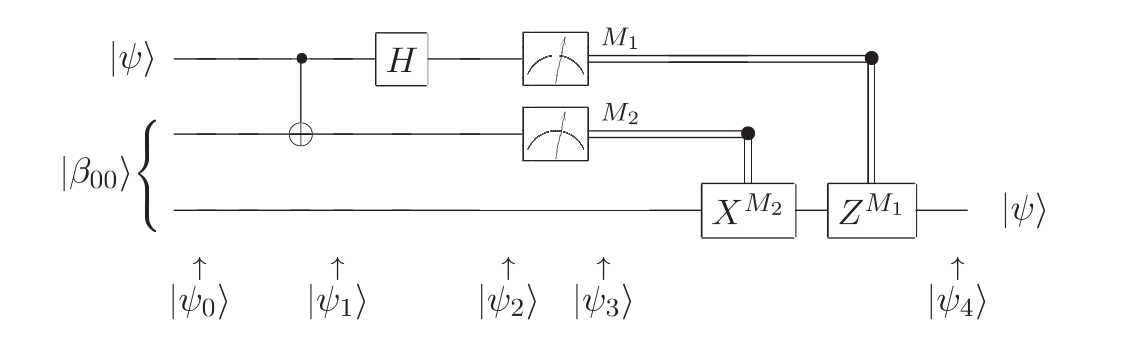
\includegraphics[width=\textwidth]{teleporation}
\end{figure}

Let's go through this circuit one by one. Observe that Alice only has the first two qubits. First a controlled CNOT operation with the qubit corresponding to the state we want to transfer as the control bit is applied.
This results in the state 
$$ \ket{\psi_1} = \frac{\alpha\ket{0}(\ket{00} + \ket{11}) + \beta\ket{1}(\ket{10} + \ket{01})}{\sqrt{2}}$$

Then a Hadamard gate on the first qubit is applied. This results in the net state being (verify that this is indeed the third state)

$$ \ket{\psi_3} = \frac{\ket{00}(\alpha\ket{0} + \beta\ket{1}) + \ket{01}(\alpha\ket{1} + \beta\ket{0}) + \ket{10}(\alpha\ket{0} - \beta\ket{1}) + \ket{11}(\alpha\ket{1} - \beta\ket{0})}{2}$$

Now this state is rather useful for us. Observe that if we measure the first two qubits, depending upon which state the first two qubits collapse into the third qubit will be one of the following states,
$$ \ket{00} : \alpha\ket{0} + \beta\ket{1}$$
$$ \ket{01} : \alpha\ket{1} + \beta\ket{0}$$
$$ \ket{10} : \alpha\ket{0} - \beta\ket{1}$$
$$ \ket{11} : \alpha\ket{1} - \beta\ket{0}$$

Thus if Alice measures the first two qubits that she possesses, depending on her result, the third qubit with Bob will change into one of the four states. If Alice passes her measurement result information (which is given in the form of two classical bits) to Bob, Bob can fix his state to obtain the state $\ket{\psi}$ back. Verify from the diagram that applying that the operations $X$ and $Z$ do indeed result in the original state reverting. For instance if the result was $11$ then Bob will apply both the $X$ and $Z$ gates while if it was $01$ then only the Z gate is applied. Thus using the EPR pair we can achieve quantum teleportation.


An important point to note here is that Quantum Teleportation does not violate the quantum no cloning theorem. Observe that we did not copy the original state to be transferred as the original state transformed into a different state losing it's initial properties. In a sense we have transferred the information, not copied it.